\clearpage
\section{Secure Multi-Party Computation}

\begin{refsection}

\begin{tcolorbox}	
\begin{tabular}{p{2.75cm} p{0.2cm} p{10.5cm}} 	
\textbf{Students Name}      &:& Mariana Ramos (02/05/2018 - 21/05/2018)\\
\textbf{Goal}               &:& Description of the problem of Secure Multi-Party Computation.\\
\textbf{Directory}          &:& \\
\end{tabular}
\end{tcolorbox}


\subsection{Problem definition}

In \textit{Secure Multi-Party Computation} (SMC) the function to be computed is defined as $(y_1,y_2,...,y_N)=f(x_1,x_2,...,x_N)$ and each party $i$ must only know (before and after the computation) its $x_i$ and $y_i$ being unknown any information about the input or output of the other parties. \cite{Naumann16}.

Thus, there are two ways of solving the problem of SMC:

\begin{enumerate}
  \item The result can be computed using a trusted party involved who has the trust from all the parties. This is a simple solution for the current problem, however, it requires a trusted party.
  \item The result can be computed without a trusted party involved using a SMC protocol. We are going to consider the \textit{Garbled Circuit Protocol} (GCP), which will have our best attention in this chapter.
\end{enumerate}

We will only focus on a two-party computation ($N=2$), with a single output, i.e. $y = f(x_1, x_2)$.

\subsection{Secure Two-Party Computation}

The \textit{Garbled Circuit Protocol} (GCP) starts with a transformation of the $f(x_1,x_2,...,x_N)$ function into a boolean circuit. The logical function $f_c$ is the output of the logical boolean circuit generator which implements $f(x_1,x_2,...,x_N)$. From the logical implementation, $f_c( )$, Alice will generate a garbled version of the logical function, $F_g^f$, as well as an encryption key $e_g^f$ and a decryption key $d_g^f$. After that, Alice's input parameter ($x_1$) and Bob's input parameter ($x_2$) must both be encrypted using the key $e_g^f$. Note that the encryption must be implemented with OT because Alice cannot know the Bob's input $x_2$ and Bob cannot know the encryption key, $e_g^f$, generated by Alice \cite{Naumann16}. Therefore after encryption Bob only gets $X_2$, which is its garbled input parameter. Next, Alice sends to Bob the garbled circuit, $F_g^f$, and its garbled input, $X_1$. With $F_g^f$, $X_1$ and $X_2$ Bob computes, the garbled output $Y_g^f$. With $Y_g^f$ and the decryption key $d_g^f$, Bob obtains $y=f(x_1,x_2)$. To conclude the protocol Bob will send to Alice the result $y$. Figure \ref{fig:garbledcircuit} shows the diagram of \textit{garbled circuit protocol}.

\begin{figure}[H]
	\centering
	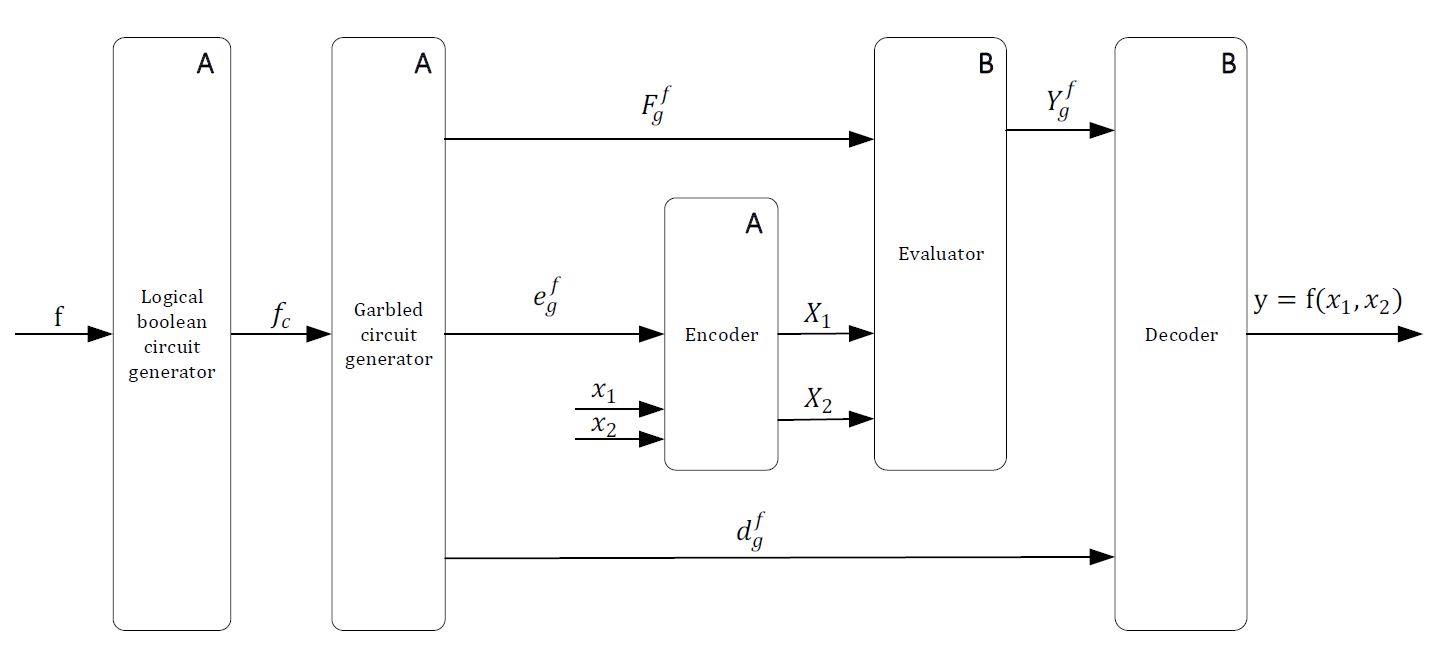
\includegraphics[width=1\textwidth, height=7cm]{./sdf/secure_multiparty_computation/figures/garbled_circuit.png}
    \caption{Block diagram of the garbled circuit protocol. Function to be computed $y=f(x_1, x_2)$. The blocks with label A are implemented by Alice and the blocks with label B are implemented by Bob.}\label{fig:garbledcircuit}
\end{figure}


\begin{table}[H]
\centering

\begin{tabular}{|c|c|}
\hline
$x_1$                   & Alice input parameter             \\ \hline
$x_2$                   & Bob input parameter               \\ \hline
$f$                     & Function to compute               \\ \hline
$f_c$                   & Logical function to be computed   \\ \hline
$F_g^f$                 & Garbled circuit of $f$            \\ \hline
$X_1$                   & Alice garbled input               \\ \hline
$X_2$                   & Bob garbled input                 \\ \hline
$e_g^f$                 & Encoding key                      \\ \hline
$d_g^f$                 & Decoding key                      \\ \hline
$Y_g^f$                 & Garbled output                    \\ \hline
\end{tabular}
\caption{Description of parameters of figure \ref{fig:garbledcircuit}.}
\end{table}




\subsubsection{Example of a two-party computation with a single output}

Lets assume:

\begin{equation}\label{eq:f_to_be_computed}
  y=f(x_1,x_2),
\end{equation}
with,

\begin{equation}\label{eq:fc_to_be_computed}
  y=f_c(x_1, x_2) = x_1 \wedge x_2,
\end{equation}
where $x_1$ and $x_2$ are single bit values. Note that even if the input parameters of $f$ and $f_c$ are represented by the same symbols they are different. The input parameters of $f_c$ are logical representations of the input parameters of $f$.

\begin{figure}[H]
	\centering
	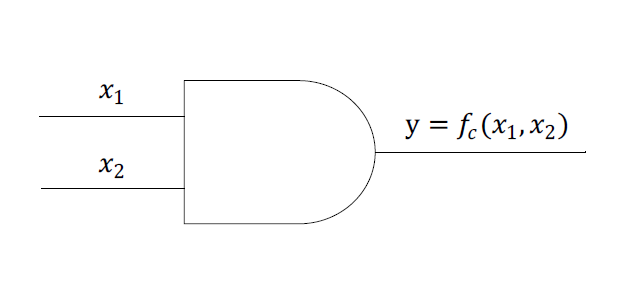
\includegraphics[width=0.4\textwidth, height=2.5cm]{./sdf/secure_multiparty_computation/figures/Gate.png}
    \caption{Gate level implementation of $f_c$.}\label{fig:andGate}
\end{figure}

Figure \ref{fig:andGate} shows the logical boolean circuit representation of the function to be computed. In this particular case there are two parties, each with an input parameter $x_i$, where $i$ can be $1$ (Alice) or $2$ (Bob), and $x_i$ can take values $0$ or $1$. Alice will play the role of \textit{garbled circuit generator} so she will generate a garbled AND gate and send it to Bob. On the other hand, Bob will play the role of \textit{garbled circuit evaluator}.

\begin{figure}[H]
	\centering
	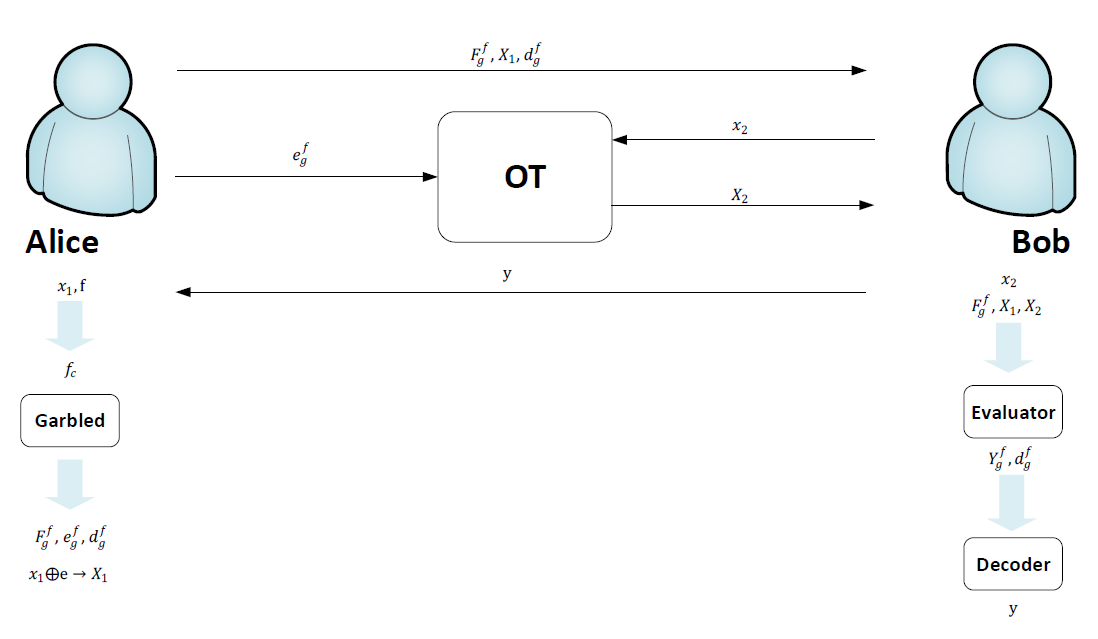
\includegraphics[width=1\textwidth, height=10cm]{./sdf/secure_multiparty_computation/figures/smc_with_ot.png}
    \caption{Garbled Circuit Protocol with OT.}\label{fig:smcwithot}
\end{figure}



\begin{table}[H]
\centering
\begin{tabular}{|c|c|c|}
\hline
$x_1$           & $x_2$             & $y=x_1 \wedge x_2$       \\ \hline
0               & 0                 & 0                             \\ \hline
0               & 1                 & 0                             \\ \hline
1               & 0                 & 0                             \\ \hline
1               & 1                 & 1                             \\ \hline
\end{tabular}
\caption{Truth table of $f_c(x_1,x_2)$.}\label{tb:truthtable}
\end{table}

Table \ref{tb:truthtable} shows the truth table of $f_c$.

Initially, Alice generates an encryption key with length equals to the sum of the length of both input parameters, two bit length in this case. Then, she encrypts her two possible input parameters, $X_1 = x_1 \bigoplus e_g^f[1]$, as well as Bob's two possible input parameters, $X_2 = x_2 \bigoplus e_g^f[2]$. 

Lets assume $e_g^f = 01$ the encryption key used by Alice. In this case, the encryption key has two bits and Alice will use the first bit to encrypt her input parameter $x_1$ and the second bit to encrypt Bob's input parameter $x_2$. We are defining the Alice encrypted input value with the label $W_1^0$ when it before encryption assumes the value $x_1 = 0$, and $W_1^1$ when it before encryption assumes the value $x_1 = 1$. The same happens for Bob, please see table \ref{tb:aliceinputs} and \ref{bobinputs}.
Now, Alice performs the encryption operation for each $x_i$, where $i \in\{1,2\}$. Regarding with Alice's input parameter, where $i=1$:

\begin{table}[H]
\centering
\begin{tabular}{|c|c|}
\hline
$x_1$           & $X_1 = W_1^{x_1}$                             \\ \hline
0               & $W_1^0=x_1 \bigoplus e = 0$                   \\ \hline
1               & $W_1^1=x_1 \bigoplus e = 1$                   \\ \hline
\end{tabular}
\caption{Encryption results for Alice's input parameter $x_1$ using the first bit of encryption key $e[1]=0$.} \label{tb:aliceinputs}
\end{table}
and regarding with Bob's input parameter $x_2$:

\begin{table}[H]
\centering
\begin{tabular}{|c|c|}
\hline
$x_2$           & $X_2 = W_2^{x_2}$                             \\ \hline
0               & $W_2^0=x_2 \bigoplus e = 1$                   \\ \hline
1               & $W_2^1=x_2 \bigoplus e = 0$                   \\ \hline
\end{tabular}
\caption{Encryption results for Bob's input parameter $x_1$ using the second bit of encryption key $e[2]=1$.} \label{tb:bobinputs}
\end{table}
Alice computes an hash using the $W_1^i$, $W_2^i$, and $y=f_c(x_1, x_2)$. 
Lets assume she computed the Hash Functions and the results are the following:

\begin{table}[H]
    \centering
    \begin{tabular}{|c|c|c|c|c|c|c|}
    \hline
    $x_1$       & $W_1^i$       & $x_2$         & $W_2^i$   &     $y=f_c(x_1, x_2)$     &    $H(W_1^i,W_2^i, y)$    &    Output                             \\ \hline
    0           & 0             & 0             & 1         &  0                        & H(0,1,0)                  & 0 0 0 0 0                             \\ \hline
    0           & 0             & 1             & 0         &  0                        & H(0,0,0)                  & 0 1 0 0 0                             \\ \hline
    1           & 1             & 0             & 1         &  0                        & H(1,0,0)                  & 1 0 0 0 0                             \\ \hline
    1           & 1             & 1             & 0         &  1                        & H(1,0,1)                  & 1 1 1 0 0                             \\ \hline

    \end{tabular}
    \caption{Hash function computed and its result.}
\end{table}

Before forwarding these values to Bob, Alice also performs an encryption over these results using a key, $d_g^f = 1 1 1 0 0$, which she'll also send to Bob. Using this encryption key the values of $\textrm{Enc}(H(W_1^i,W_2^i,f_c )) = H(W_1^i,W_2^i,f_c) \bigoplus d_g^f $ are the following:

\begin{table}[H]
    \centering
    \begin{tabular}{|c|c|}
    \hline
    Enc($H(W_1^0,W_2^0,0)$)             &    1 1 1 0 0                                      \\ \hline
    Enc($H(W_1^0,W_2^1,0)$)             &    1 0 1 0 0                                     \\ \hline
    Enc($H(W_1^1,W_2^0,0)$)             &    0 1 1 0 0                                     \\ \hline
    Enc($H(W_1^1,W_2^1,1)$)             &    0 0 0 0 0                                     \\ \hline
    \end{tabular}
    \caption{Encrypted hash results.} \label{tb:encryptedhash}
\end{table}
 Now the rows of table \ref{tb:encryptedhash} must be permutated randomly \cite{Yakoubov}. 

\begin{table}[H]
    \centering
    \begin{tabular}{|c|c|}
    \hline
    Enc($H(W_1^0,W_2^1,0)$)             &    1 0 1 0 0                                     \\ \hline
    Enc($H(W_1^1,W_2^1,1)$)             &    0 0 0 0 0                                     \\ \hline
    Enc($H(W_1^0,W_2^0,0)$)             &    1 1 1 0 0                                     \\ \hline
    Enc($H(W_1^1,W_2^0,0)$)             &    0 1 1 0 0                                     \\ \hline
    \end{tabular}
    \caption{Permutated Garbled Output}
\end{table}


\begin{table}[H]
    \centering
    \begin{tabular}{|cc|c|}
    \hline
    $W_1^i$ & $W_2^i$   & Enc(H($W_1^i$,$W_2^i$,f ))         \\ \hline
    0       & 1         & 1 1 1 0 0                          \\
    0       & 0         & 1 0 1 0 0                          \\
    1       & 1         & 0 1 1 0 0                          \\
    1       & 0         & 0 0 0 0 0                          \\ \hline
    \end{tabular}
    \caption{Garbled Circuit.}
    \label{tb:summary}
\end{table}
Alice sends to Bob the garbled circuit, which is a circuit capable of generate the table \ref{tb:summary}. Alice also sends to Bob, $d_g^f$. With $W_1^i$  and $W_2^i$ that Bob already has, he computes the circuit output. He decrypts this output doing $\textrm{output} \bigoplus d_g^f$ . After, he also tries all possible outputs, doing $H(W_1^i, W_2^i, \textrm{guess Y})$ being the one that works, the right one.

Both Alice and Bob must follow the \textit{oblivious transfer protocol} in order to Bob gets his garbled version of his input, $X_2$. In this case, lets assume that Bob's input parameter is $x_2=1$. This way, Alice sends to Bob using OT $W_2^1=0$.  With both inputs garbled versions, Bob can perform a \textrm{XOR} operation between the equivalent result of $\textrm{Enc}(H(W_1^i,W_2^i,f_c ))$ and the decryption key $d_g^f$:

\begin{equation}\label{eq:decryptiongarbled}
  \textrm{Enc}(H(W_1^i,W_2^i,f_c ))\oplus d_g^f = 0 1 0 0 0.
\end{equation}
Since Bob knows $X_1 = W_1^i$, $X_2=W_2^i$ and the result of $\textrm{Enc}(H(W_1^i,W_2^i,f_c ))$, he must introduce this information in the Hash Function in order to get $y=f_c(x_1,x_2)$. Thus, he will discover the output value $y=0$ without learning anything about the input parameter introduced by Alice. Nevertheless, since an oblivious transfer protocol was used to send to Bob his garbled version of his input parameter, Alice also knows anything about the input parameter introduced by Bob.

\newpage

\subsection{TinyGarble}
	
This subsection will cover \href{https://github.com/esonghori/TinyGarble}{TinyGarble}, a GC framework that allows two parties to safely compute any function with their private inputs through Yao's Garbled Circuit Potocol.
With TinyGarble it's possible to use both High Level Languages and Hardware Design Languages as input formats. With the former, High Level Synthesis (HLS) will be needed to convert the high level language into HDL, some tools that can be used are SPARK or Xilinx Vivado, for C.
With HDL inputs, like VHDL or Verilog, a  RTL Synthesis tool like Yosys-ABC, along with TinyGarble's custom libraries, have to be used in order to generate a Netlist file. This file then has to be translated into a simple circuit description file (SCD) with the help of TinyGarble's converter.
Once the SCD file is generated, it can be provided to and executed by both parties.

\begin{figure}[H]
	\centering
	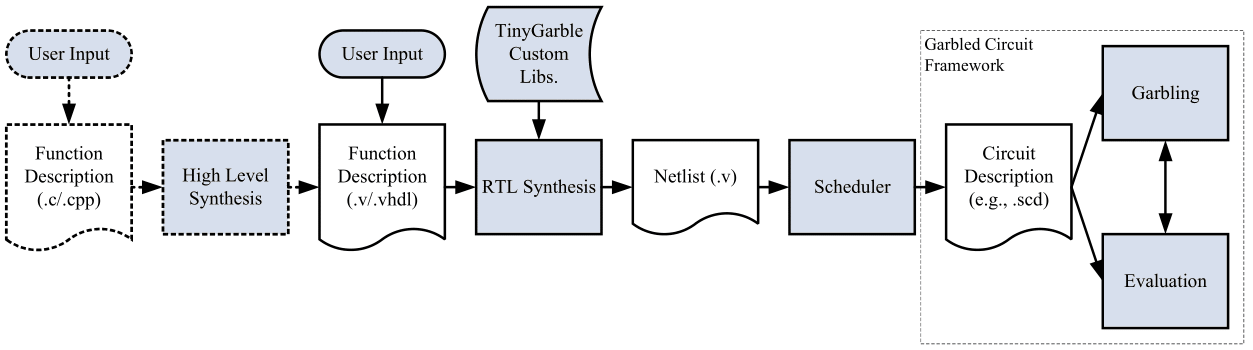
\includegraphics[width=1\textwidth, height=4cm]{./sdf/secure_multiparty_computation/figures/tiny_garble_flow.png}
    \caption{TinyGarble Global Flow\cite{Songhori}}\label{fig:tinygarble_flow}
\end{figure}

In terms of performance, when using HDL input directly, the end circuit will have considerably less logical gates, depending on the function, than when using high level languages inputs, since these last ones need an extra step of synthesis. The table below shows the comparison between the performance of the circuits generated with
C input to Verilog using a HLS tool, and a Verilog input.

\begin{figure}[H]
	\centering
	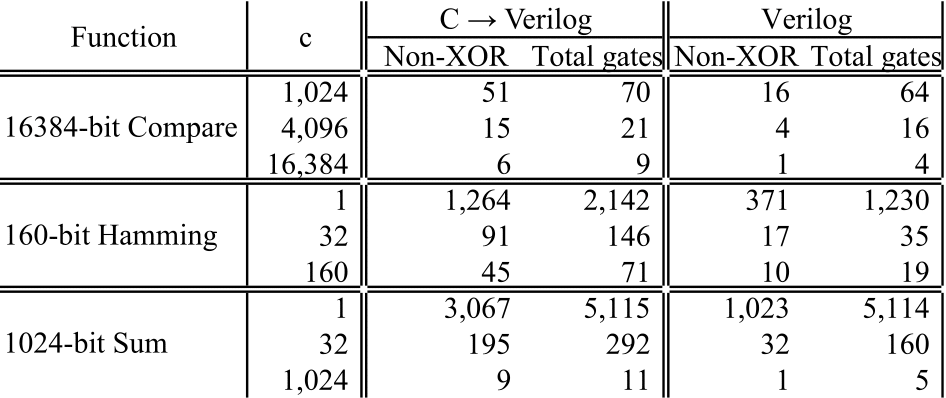
\includegraphics[width=1\textwidth, height=5cm]{./sdf/secure_multiparty_computation/figures/tiny_garble_CvsHDL.png}
    \caption{Performance comparison between C and Verilog input\cite{Songhori}}\label{fig:tinygarble_comparison}
\end{figure}

\newpage

Below it's the implementation of an 'And' function with TinyGarble.
First the verilog/vhdl code is written.

\begin{lstlisting}[caption={and\_gate.v}, language=Verilog] 
module and_gate (input a, b, output y);
	assign y = a & b;
endmodule
\end{lstlisting}

Then, following TinyGarbles' isntructions for Yosys (The RTL Synthesis tool mensioned above) to compile the verilog file into a netlist verilog file, the following output was produced:

\begin{lstlisting}[caption={and\_gate\_netlist.v}, language=Verilog] 
(* top =  1  *)
(* src = "and.v:1" *)
module and_gate(a, b, y);
  (* src = "and.v:2" *)
  input a;
  (* src = "and.v:2" *)
  input b;
  (* src = "and.v:3" *)
  output y;
  AND _0_ (
    .A(b),
    .B(a),
    .Z(y)
  );
endmodule
\end{lstlisting}

The next step would be to convert the netlist file into a SCD file, but TinyGarble's converter was failing in middle process with Segmentation Fault error.
Looking back at the netlist file, there are some noticeably weird lines, starting with "(*", removing those lines fixed the Segmentation Fault problem, but the SCD file wasn't being generated.
Checking the log files, the converter was complaining about invalid input and output names, it needed (p\_init, g\_init, e\_init, p\_input, g\_input, e\_input) as input name, and (o, terminate) as output name.
Fixing everything the final netlist file looked like the following:

\newpage

\begin{lstlisting}[caption={and\_gate\_netlist\_fix.v}, language=Verilog] 
module and_gate(p_input, g_input, o);
  input p_input;
  input g_input;
  output o;
  AND _0_ (
    .A(g_input),
    .B(p_input),
    .Z(o)
  );
endmodule
\end{lstlisting}

Even though the SCD file was finally generated, it was producing wrong outputs when executed by Alice and Bob:

\begin{figure}[H]
	\centering
	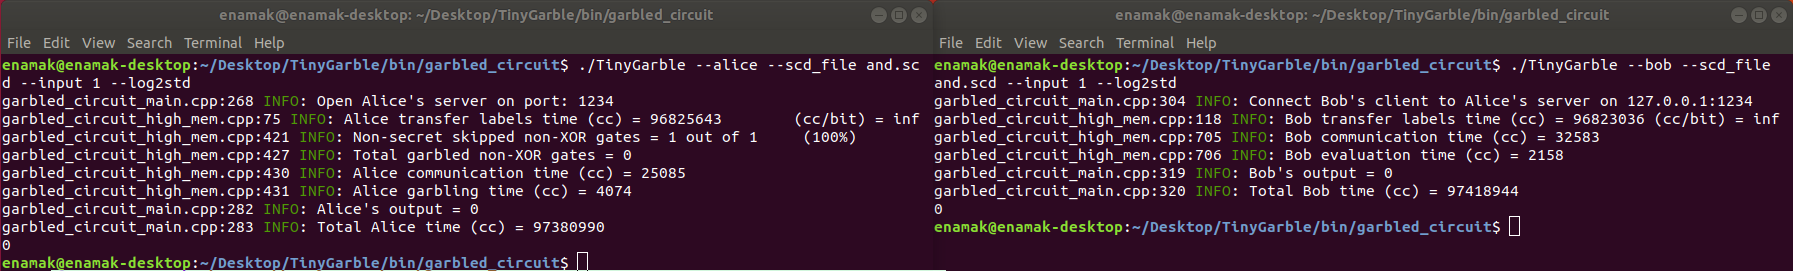
\includegraphics[width=1\textwidth, height=4cm]{./sdf/secure_multiparty_computation/figures/tinygarble_terminal.png}
    \caption{And function executed by Alice and Bob with TinyGarble}\label{fig:tinygarble_terminal}
\end{figure}

% bibliographic references for the section ----------------------------
\clearpage
\printbibliography[heading=subbibliography]
\end{refsection}
\addcontentsline{toc}{subsection}{Bibliography}
\cleardoublepage
% -------------------------------------------------------------------- 